\chapter{Вольга и Выбуты}

Связь Ольги с «весью Выбутовской» заслуживает отдельного разговора, хотя и не касается Киева. Согласно некоторым житиям Ольги, родилась она в «веси Выбутовской» или «Выбуто». «Весь» это деревня, небольшое село. Вроде там же Игорь встретил юную Ольгу, перевозчицу на лодке, хотя рассказ сей относится к той смутной временной области летописных и житийных преданий, листы которой вынуты из Лаврентьевской летописи. 

Деревни Выбуты в Псковской области нынче нет. Пре\-жде существовал Выбутский приход, названный по имени селения, и некоторые полагают, что село Выбуты находилось там, где ныне на возвышенном каменистом, покрытом травой правом берегу реки Великой стоит церковь Ильи Пророка с кладбищем при ней, чуть к западу.

Церковь построена в 14 или 15 веке, будто бы взамен старинной деревянной, что была «тремя годами старше самого Пскова». До конца 20 века держалось предание, что когда возвели каменную церковь, деревянная еще стояла рядом и народ ходил именно туда, презрев новое здание. Посему деревянный храм сожгли.

Именно это место, с каменной церковью и кладбищем слывет теперь Выбутами, или погостом Выбуты. Инспектор Псковской семинарии и краевед Александр Князев в 19 столетии считал, что при Выбутской церкви некогда хранились сани княгини Ольги, однако след их утерян.

Течет река Великая, чем-то напоминающая Десну по виду и ширине. Две деревни одна против другой, через воду – Кузнецово и Волженец\footnote{57°42'8"N 28°14'59"E}. 

Местность Выбуты лежит в километре к востоку от Кузнецово по тому же берегу. От Кузнецово к Волжецу через реку есть основы разрушенного еще в Великую Отечественную войну моста, а также используемый Литовский брод, который можно переехать на машине или велике. Дно у брода – из каменных плит. Это особенность реки на участке вдоль Выбут и Волжеца, ибо дно песчаное сменяется здесь выходом известняковой породы. Жители Волжеца вброд переходят Великую на сторону Кузнецово, дабы сесть на 107-й автобус, что ездит в Псков. Также, по пояс в воде, можно перебраться через Ольгины пороги – еще одну приподнятую каменную гряду. Значит, в старину здесь можно было переправляться без мостов. Киев тоже находится там, где Днепр в иные годы переходили вброд. Именно по таким местам пролегали пути кочевников и торговцев во времена, когда люди не умели строить мосты. 

\begin{center}
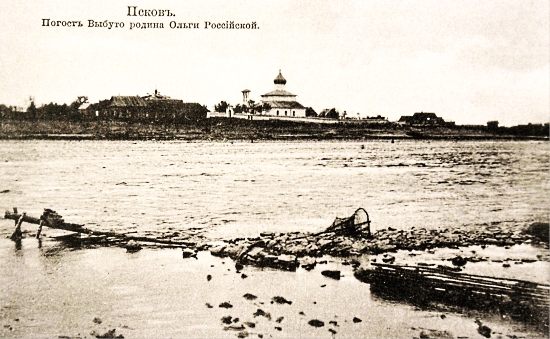
\includegraphics[width=\linewidth]{chast-volga/vybuty/olga02.jpg}

\textit{Вид на церковь Ильи и погост. Дореволюционная открытка.}
\end{center}

\newpage

\begin{center}
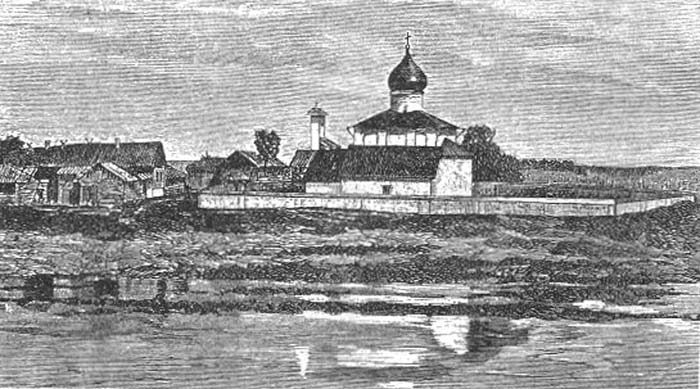
\includegraphics[width=\linewidth]{chast-volga/vybuty/vybuty-01.jpg}

\textit{Церковь Ильи, картинка из «Русского паломника» 1914 года.}
\end{center}

На страницах летописей, Ольгины (Выбутские) пороги возникают в связи с их защитой войсками псковитян, ибо через место сие проходила дорога на южные околицы Пскова, посад Полонище. Прорыв врага здесь, на переправе, грозил захватом Полонища и прямым подступом к укрепленной части Пскова.

Как обычно в местностях крайне важных для истории, в районе Выбутов, к северу, имеется заполненный водой карьер, где относительно недавно добывали камень для строительства. На восток – такой же выход каменной породы, еще неразработанный. 

А Ольгинские пороги – точно напротив церкви Ильи. Через реку они касаются деревни Паничьи Горки, а на запад по дороге недолго идти до Волженца, где проживает всего около 20 жителей. 

Прежде его кликали еще Выдрой и Волжино, а также – деревня Вольжина или Вольгина. Волжино – значит Волги. Предположу, что ей это селение принадлежало. Потому и Волжино. Сразу рассуждение, что именно под именем Волги, с «В» в начале, и была известна тут Ольга во время своего владения деревней.
%
%Деревня Выдра- Ольжина ( Ольженець.jpg
%
Что до Выдры, то рядом со старой деревней Волжиной было меньшее селение, Выдра, в 19 веке поглощенное Волжиной. И какое-то время эти совмещенные деревни назывались одним именем – Выдра, хотя население продолжало считать себя жителями Волжиной и Выдры раздельно.

\begin{center}
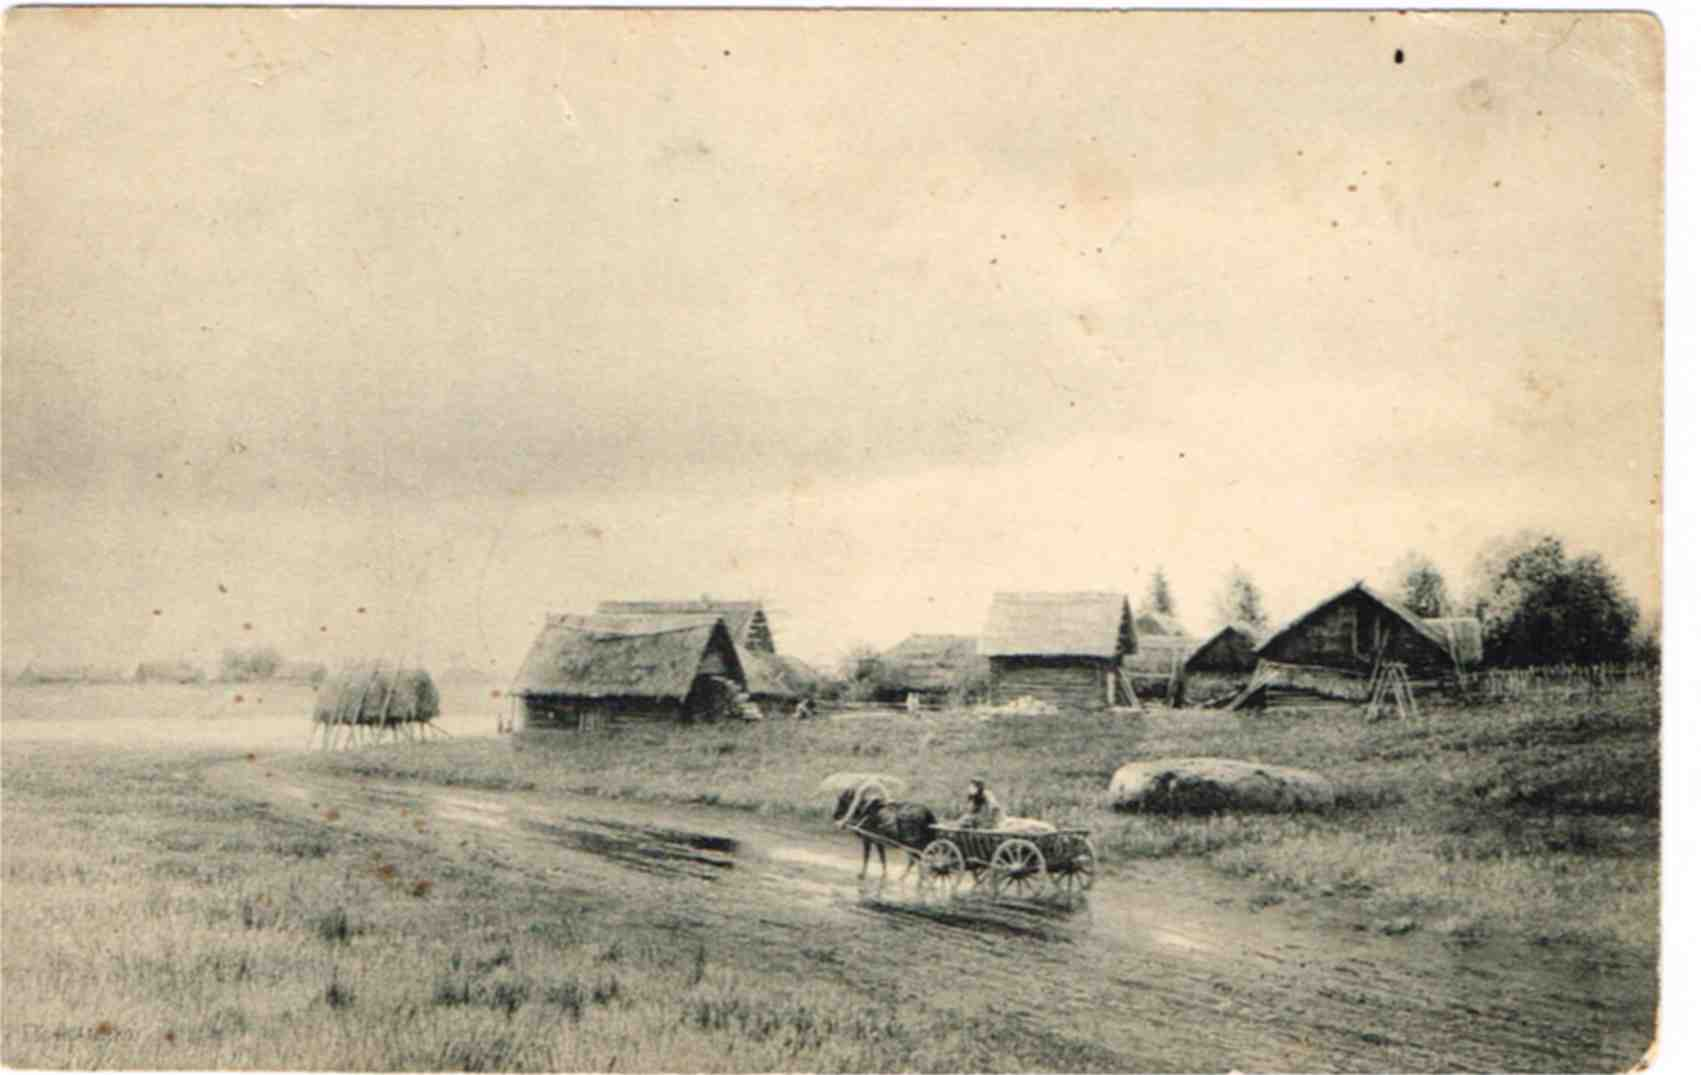
\includegraphics[width=\linewidth]{chast-volga/vybuty/vydra.jpg}

\textit{Деревня Выдра до революции.}
\end{center}

В 1874 году туда отправился барон Николай Богушевский и написал «Заметку о селе Выбутах (Лыбутах)», опубликованную во втором томе «Труды археологического съезда в Киеве (1874)», издания 1878 года. В ней он собрал местные предания, относящиеся к Ольге.

Представления крестьян насчет точной родины Ольги разделялись. Одни полагали, что Ольга родилась в деревне Горе (Горке) – ныне это, вероятно, Паничьи Горки\footnote{Панами в северных преданиях 19 века называли «чудских начальников», всю чудь вообще, а иногда просто каких-то давних, позабытых неприятелей – понятие от местности к местности разнилось.}, с постоянный населением 5 человек на начало 21 века. Другие же указывали на Волжино.

На берегу реки, около 25-30 саженей (53-64 метра) выше по течению от Вольжиной (значит, на запад), среди поля, барон видел развалины, считающиеся Ольгиной церковью или её дворцом. Вот что он пишет:

\begin{quotation}
видны полузасыпанные землею развалины, древнего, грубо – из ручного известняка – сложенного фундамента. Здание, от которого сохранились эти развалины, имело очевидно форму правильного параллелограмма, узкие стороны которого обращены к востоку и западу – а внутренность разделена на пять отделений: из них два больших, и три маленьких. Длина всего здания около восьми, а ширина около шести саженей.

Крестьяне считают это место святым, не распахивают его – хотя оно находится посреди поля – и намереваются устроить на развалинах часовню в честь святой благоверной великой княгини Ольги, дворец которой (а по сказанию иных церковь её, разоренная «поганой Литвой») стояла на этом месте. Тут же – где-то находился сад и погреба великой княгини – «наполненные золотом и серебром», но найти или видеть их можно только в ночь на Ольгин день (11-го июля) – так как святая Ольга была «великая колдунья» и наложила на свои сокровища и сады чары, превратившие её любимую усадьбу в «усадьбу невидимку».
\end{quotation}

Невидимые дворцы и сады! Ведь это излюбленная тема в сказаниях о Туаха Дэ Дананн, об эльфах, фэйри, хулдуфолк.

Невидимость их распространялась на живое и неживое. Были определенные условия невидимости – например, в ирландском предании «Воспитание в домах двух чаш» на героев из числа «чудесного народа», действуют некие чары Фет Фиада, которые обеспечивают «невидимость» героев от восприятия людей. Когда же чары рассеиваются, героиня по имени Этне перестает видеть своих волшебных подруг, а сама становится видимой людям и вступает с ними в общение.

Вспомним про ши (sidhe) – незримые жилища, крепости эльфов, фомойри, скрытого народа (хулдуфолк). До сих пор исландцы считают, что там, где человек воспринимает органами чувств некие руины, для скрытого народа там же находятся вполне целые дворцы или крепости. Это представление в точности совпадает с представлением русских крестьян о дворце Ольги!!!

Для исландца с мировоззрением в духе его культурной традиции, развалины дворца Ольги – классический ши! А кто владельцы ши? Представители скрытого народа. Как и крестьяне Волжино в 19 веке, исландцы по сей день чтут ши свято, даже дороги прокладывают не по руинам хулдуфолка, а в обход.

\begin{center}
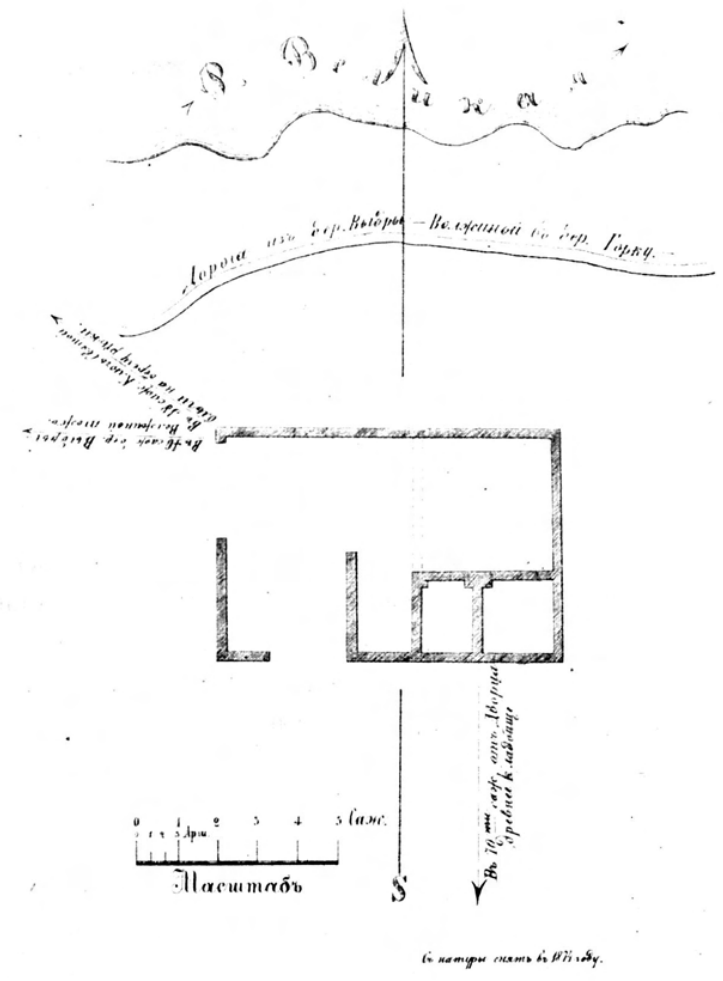
\includegraphics[width=0.92\linewidth]{chast-volga/vybuty/volga-dvorec.png}

\textit{План «дворца Ольги», составленный Богушевским.}
\end{center}

Сейчас приезжим туристам показывают сие место метрах в 200 по дороге от того места, где Ольгин ключ на берегу реки, а потом несколько западнее – но это противоречит сведениям Богушевского. Существует еще мнение, что руины были там, где в наше время поставили киот (будочка на столбе, с иконой)\footnote{57°42'10"N, 28°15'12"E}, в 111 метрах на восток от Ольгина ключа. 

Но вернемся к заметке барона:

\begin{quotation}
Неподалеку от развалин «дворца» находится древнее кладбище и группа могильных насыпей (курганов), в которых иногда находятся черепа, кости и обломки доспехов и оружия. 

Не берегу реки из-под отвесной известковой скалы струится прозрачный как хрусталь и холодный как лед источник: так называемый «Ольгин ключ».
\end{quotation}

По преданию, сюда юная Ольга приходила умываться и вода в роднике\footnote{57°42'10"N, 28°15'5"E} от того стала целебной. Как бы ни было, в 19 веке источник посещали богомольцы, бросали туда монеты, а крестьяне эти монеты собирали. Уже ко времени посещения сих мест Богушевским, желающих исцелиться стало совсем мало. 24 июля 2011 года, точно в Ольгин день (по новому стилю) родник иссяк. К 14 октября вода снова пошла, но уже в меньшем количестве.

Богушевский пишет:

\begin{quotation}
Не более как в 150 саженях к северо-востоку от Выбут – за деревенькой Беклеши – на пустынном низменном лугу, окруженном с трех сторон песчаными холмами, покрытом огромными обломками и изрытом глубокими ямами, возвышается громадная гранитная глыба – продолговатой формы, имеющая в длину до восьми, а в высоту и ширину до трех аршин. Глыба эта считается святою и называется «Ольгиным камнем». Почему эта громадная скала считается святою и носит имя святой Ольги – я никак не мог узнать.
\end{quotation}

Беклешей как отдельного селения больше нет. Одно время оно называлось еще то Першино, то Веригино. Потом его поглотило село Бабаево, ныне существующее менее чем в полукилометре на восток от Выбутов. Остатки взорванного (разрушена верхняя половина) в 1960-х Ольгиного камня покоятся в 300 метрах от Бабаево, около южной части Выбутского карьера.

\begin{center}
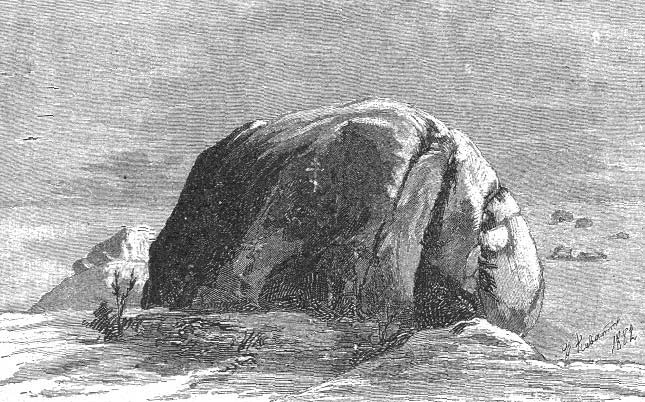
\includegraphics[width=\linewidth]{chast-volga/vybuty/vybuty-olgin-kamen.jpg}

\textit{Ольгин камень, картинка из «Русского паломника» 1914 г., рисунок 1882 г.}
\end{center}

Своё сообщение о камне Богушевский дополнял вот чем:

\begin{quotation}
Впрочем в народе существует следующее баснословное предание: «однажды святая Ольга, торопясь в Выбутскую церковь к заутрени, услышала, что уже кончили благовестить – и опасаясь опоздать, бросила на поле большой камень, который несла в рукаве. [...]

Есть еще другой, следующий вариант этой легенды: когда святая Ольга отправлялась на «войну с поганью», то несла в «платке» множество больших камней, на пол-дороги платок прорвался и из него выпал большой камень. [...]

Далее рассказывают, что когда строился мост для Санкт-Петербургско-Варшавской железной дороги через близлежащую реку Череху, то Ольгин камень сверлили и хотели разорвать порохом, но никак не могли; «видно святая не дала» говорит народ.
\end{quotation}

%Богушевский делает также примечание:

%\begin{quotation}
%На правом берегу р. Кеби, впадающей в р. Череху – недалеко от слияния Черехи с Великой – есть место называемое Буденик, где некогда по преданию жила св. Ольга и где родился внук ее в. кн. Владимир Святославович. (Князев. Указатель достопамят. города Пскова стр. 40)
%\end{quotation}

В «Указателе достопамятностей города Пскова», составленного Александром Князевым, издания 1858 года, сказано:

\begin{quotation}
Несколько ниже Лыбут на р. Великой есть остров, разделяющий ее на два рукава. Один из этих рукавов называется «Ольгиными слудами» (слуды – подводный камень) и другой «Ольгиными воротами». Ниже этих ворот, на правом берегу реки Кеби, впадающей в р. Череху, есть место, называемое Буденик, где некогда, по преданию, жила Св. Ольга и где родился внук ея, В. К. Владимир Святославич.
\end{quotation}

Было еще две легенды о камне. Первая, что Ольга поставила его там, где хотела указать людям на место для возведения храма. И вторая – Ольга несла его к мосту, что она строила, но услышав звон колокола к литургии, оставила камень и поспешила в церковь. Ходило также предание, что Ольга была «сильной богатыркой» и переносила здоровенные камни. Я не могу найти само предание целиком, записанное Василием Ильичем Чернышевым в 1917 году.

Рядом с этим камнем в 1883 году поставили кирпичную часовню «Ольгин крест» и водили к нему паломников. На камне же, по крайней мере с начала 20 века, показывали «следы стоп» Ольги – два отпечатка босой детской или женской ноги. Богушевский про них однако ничего не написал, из чего можно сделать вывод – или по какой-то причине барон не упомянул про следы, либо следов тогда не было, их выбили в камне позже. 

Следы ступней в камнях имеют отражение в легендах всех континентов. Такие следы приписывают богам, святым, чуди белоглазой, чертям и народным героям. К слову, в окрестностях Выбутов и близких мест много так называемых камней-следовиков – валунов с некими искусственными выемками. В Пскове на площади Победы, в Выбутах – к востоку от церкви Ильи, а также в малиновых кустах «справа от Ольгиного камня», и на этом следовике – детского размера след ступни с узкой пяткой, без пальцев.

Ольгин камень в советское время взорвали, сейчас паломникам и туристам показывают вроде бы его остатки – зацементированную груду камней с водруженным в 1993 году сверху крестом. А Ольгину часовню разобрали местные жители.

Богушевский описал и второй Ольгин камень. Он был саженях в двадцати от Шацкого острова. Эдак в километре к востоку от Выбутов, короче говоря напротив Бабаево, река Великая расширяется, и в ней из воды выступает множество каменистых, поросших травой островов, наибольший из которых зовется Шацким по имени его давнего владельца. Сейчас этот остров называют еще Богдановским. Северная, или правобережная протока от него – мелкая, Ольгины слуды. Левобережное, южное русло – Ольгины ворота. К западу от Шацкого острова

\begin{quotation} 
выдвигаются из воды несколько громадных гранитных камней. Один из них называется «Ольгиным». Предание говорит, что когда святая Ольга купалась в реке, то после купанья, камень этот служил ей местом отдохновения.
\end{quotation} 

Однако в наши дни старожилы вспоминают некий  Ольгин камень еще в другом месте. 

Примерно до середины 20-го века, под обрывом берега чуть выше по течению от Выбутской церкви, то есть под тем местом, где кладбище, лежал валун двое меньший того, что у Беклеши, и на нем был след ноги 36-37 размера. Этот камень тоже назывался Ольгиным.

Судя по тому, что про «второй» Ольгин камень Богушевского сейчас не говорят, а «третий» тоже лежит в реке, быть может, несмотря на некоторое между ними расстояние, речь идет об одном камне. Однако, Богушевский и касательно своего «второго» ничего не писал о следе ноги.

\begin{center}
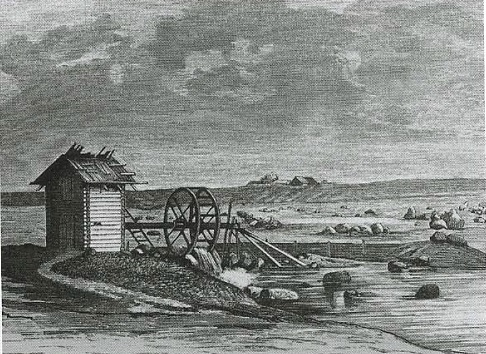
\includegraphics[width=\linewidth]{chast-volga/vybuty/sludy2.jpg}

\textit{1883. Ольгины ворота и Ольгины слуды на реке Великой. Гравюра с наброска Г. Пиватто.}
\end{center}


В Псковском музее были литография и гравюра конца 19 века, связанные с Выбутами, неизвестного художника. Во время войны немцы их украли, и остались только две плохие фотокопии. Описание картины «Вид Ольгиных слуд в погосте Выбуте» следующее:

\begin{quotation}
Вид реки Великой с частью берега; в левой части показаны запруда у берега, небольшой домик водяной мельницы с решетчатым водяным колесом и камни в реке. Левее домика, в перспективе – ещё один. На противоположном возвышенном берегу видны крыши деревни. Внизу, в центре и справа – тёмная часть берега; гравюра не идентична подобной ей 1882 г. («Всемирная иллюстрация», 1883 г.)
\end{quotation}


\begin{center}
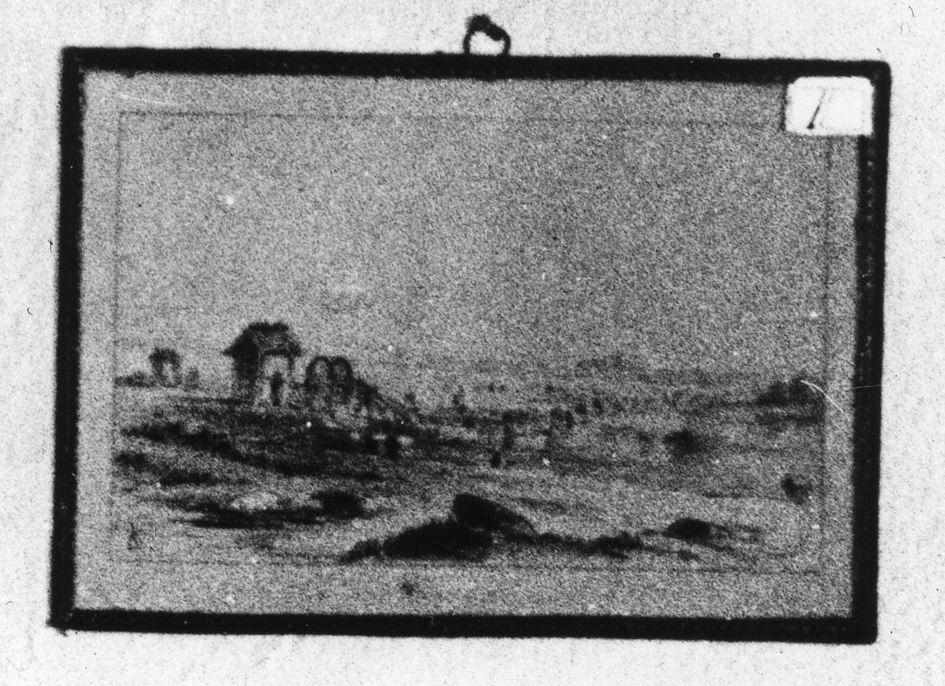
\includegraphics[width=0.90\linewidth]{chast-volga/vybuty/vyb-sludy.jpg}

\textit{Вид Ольгиных слуд в погосте Выбуте.}
\end{center}

\begin{center}
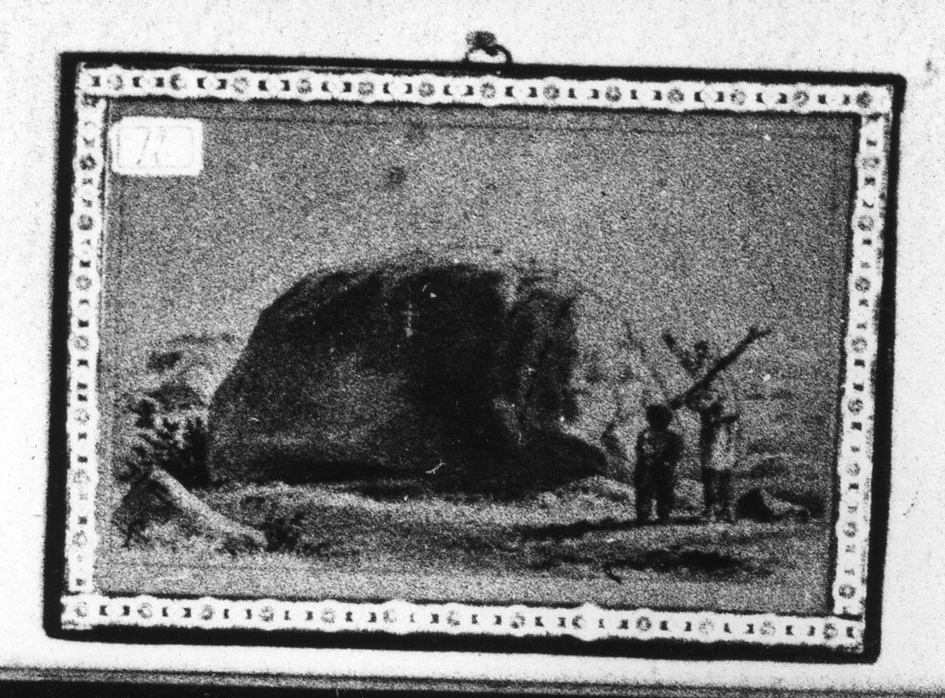
\includegraphics[width=0.90\linewidth]{chast-volga/vybuty/vyb-olgin-kamen-02.jpg}

\textit{Ольгин Камень возле погоста Выбуты.}
\end{center}

\newpage

А что официальная наука? Археологи раскопали Выбуты вдоль и поперек, впрочем мне неизвестно об исследовании развалин Ольгиного дворца. Некоторые из разбросанных по округе курганов имели в основании своем каменные цоколи. Это позволяло им веками сохранять форму, не расползаться.

Местность была обжита издревле, наибольшее поселение найдено в районе Выбутского погоста. Наиболее ранний слой ученые датируют от 500 года и выше, позднего – 18 век. Есть и захоронения примерно 1-2 веков нашей эры. На этот счет существуют работы, разбросанные по публикациям в различных малотиражных сборниках и по рукописям в архивах.

В августе 1859 года на Псковщине побывал Павел Якушкин, чьими «Путевыми письмами из Новгородской и Псковской губерний»\cite{yakushin01} мы уже пользовались относительно «змияки Перуна». Якушкин в Пскове взял челнок и попутчика, здешнего старика Алексея Федоровича Полякова. Они поплыли вниз по реке Великой, осматривая окрестности. Якушкин впитывает в себя народные, не книжные названия, и передает их читателю. Не Псков, но Опсков\footnote{В летописях же Псков называется Плесков.}. Озеро Псковское, куда впадает Великая, все зовут Талабским – как не вспомнить тут наше Долобское и не услыхать между ними сходство?

Якушкин и Поляков едут рекой назад в Опсков:

\begin{quotation}
 – Вот здесь был городок, – сказал мне Алексей Федорович, указывая не левый берег Великой, когда мы немного проехали погост Устье и Назимовскую гору.

 – Чей же такой город был?

 – Говорят – царицы Ольги, – отвечал он, – да тому нельзя быть.

 – Почему же?

 – За что, а за то: этот берег (западный) весь край \textit{забранный}; да и этот (восточный) пустой был. На нашей стороне был Сороковой бор, и в том бору жил вольный народ: холоп беглый, так-какой грешник (преступник). Заберут в какую деревню: прикажут пиво варить; а не то – грабить.... Бывало, поймают которых – вешать. бабка моя жила 120 лет, сама видела виселицу в Чертовом Ручью, что для такого народа была сделана... Война была частая: то Швед подойдет, то Литва, то Немец из-под Риги; пройдут, да вплоть до самого Опскова и вычистят; ну, до Опскова вычистят, а в самый Опсков ни разу никто не входил, ни один злодей. А остатняя война Шведская: дошел Швед до Печор – да и полно! А прежде Литовский царь Баторий подступал: на Терехе в монастыре Пантелеймоновом шатры разбивал; в Лыбуте, 17 верст вверх по воды, прямо переправлялся со всею своею силою.

 – Лыбута\footnote{Здесь Якушкин делает примечание: «Говорят и Лыбуста, но Выбутой не называют, как в одной книжке сказано».} город или село?

 – Нет, просто деревня.

Надо заметить, что здесь погостами называют сёла, селом – сельцо, т.е. где есть барский дом; а деревнею – где нет ни церкви, ни барского дома.
\end{quotation}

Прервем чтение заметок. Сам Якушкин в Выбутах не побывал и пересказывает слова осведомленного попутчика. Остается неясным, в самом ли деле существовало селение Выбуты по крайней мере по середину 19 века, или Поляков говорит о старине, что Лыбуты существовали в 16 веке при Баторие.

Далее, то ли Поляков был кладезем местных преданий, то ли Якукшин складно вложил в его уста всё, что слышал среди здешнего народа про Ольгу. Повествование это любопытно для сравнения с летописными и житийными сведениями:

\begin{quotation}
 – Только эта деревня знатна гораздо за тем: в той деревне Лыбуте родилась царица благоверная Российская Ольга; родилась она в крестьянском звании и была перевозчицей; а за тем, что горазд из себя красавица была, да и горазд хитра была – царицей сделалась, а там во святые вошла.

 – Как же так это случилось?

 – А вот слушай: с первоначалу жизни, немного по после, была, как сказано, Ольга крестьянка перевозчицей в Лыбуте. Раз перевозит она князя Всеволода\footnote{Около Пскова и Новгорода в тридцатых годах 12 века крутился Всеволод Мстиславович. Так, к слову.}...

 – Какой такой князь Всеволод?

 – Всеволод, да и Всеволод, нее знаю. Увидал Всеволод Ольгу и помыслил на Ольгу; а этот князь был женат. Стал тот князь говорить Ольге, а Ольга ему на те его на пустыя речи ответ: «Князь! Зачерпни рукой справа водицы, испей!». Тот зачерпнул, испил. «Теперь», – говорит Ольга, «теперь, князь, зачерпни слева, испей и этой водицы». Князь зачерпнул и слева водицы, испил. «Какая же тут разнота: та вода и эта вода?» – спрашивает Ольга у князя. «Никакой тут разноты нет», – говорит князь, «всё одна вода». «Так», – говорит Ольга, «что жена твоя, что я, для тебя всё равно». Князь Всеволод зарделся, замолчал и отстал от Ольги. Да и много она князей перевела: которого загубит, которого посадит в такое место... говорят тебе: горазд хитра была. Спустя сколько времени Ольга пошла за князя замуж, только не за Всеволода, а неизвестно за какова. Тогда много князей было, и всякий своим царством правил, а все между собой родня были и все промеж себя воевали: хотелось всякому у другова царство его отнять. Пошел войною на мужа Ольгинова его двоюродный брат, да и убил его. Убил мужа Ольги, да и прислал к ней послов мириться: только Ольга которых посадился за стол обедать, да и приволила их в волчью яму, что под тем столом вырыта была; а которых зазвала в баню, а там обложила баню хворостом, да и сожгла всех, а после самого их князя убила, на его царство села и стала двумя царствами править. Прошло сколько времени, поехала Ольга в Царь-город к тамошнему царю в гости. Как увидал ее тамошний царь: «Выходи», – говорит, «за меня замуж!». Ну, а Ольге какая неволя была идти замуж? Сама себе царица! А выйди замуж: муж глава жене. «Ты», – говорит Ольга, «православный, а я поганая (она тогда не крестимшись была), так мне не приходится за тебя идти». «Ну, так крестись», – говорит царь. «А ты будешь моим крестным!». «Хорошо!», – говорит. Перекрестилась Ольга, приняла крещеную веру. «Теперь давай венчаться», – говорит царь. А Ольга ему: «Нельзя – ты мой крестный!». Так и провела.
\end{quotation}

По ходу чтения у меня вдруг возникло обоснование сомнения про житийное предание о лодочнице Ольге. Перевозят – где глубоко. А возле Выбутов – брод, естественная переправа.

От Пскова Якушкин поехал в лежащий за тридцать километров летописный Изборск. Хотя по летописям там княжил брат Рюрика, Трувор, местное население однако не раз говорило путешественнику, что княжил сам Рюрик. 

Татищев же в «Истории» утверждал, что Изборск именовался Ологиягард от княгини Ольги, да вытащил на свет еще одно название иноземное – Алогиябург (Alogiaborg), которое швед Филипп-Иоганн Страленберг (Philipp Johann von Strahlenberg) в книге на немецком языке «Das Nord- und ostliche Theil von Europa und Asia» сопоставлял со Старой Ладогой, хотя по мнению Татищева, ошибочно.

А от Изборска в пятнадцати километров – поселок Печоры, названный так, подобно нашему Печерску, от пещер. Есть там и Псково-Печерский монастырь с древними пещерами. 

«Новый и полный географический словарь России» 1788 года насмешливо и кратко передавал предание о подземном ходе из Печор в Киев.

Якушкин записал подробнее:

\begin{quotation}
 – Давно, еще за Грозного царя, – стал говорить мой собеседник, – были в Изборске отец с сыном, оба благочестивые люди и охотники на птицу, на зверя ходить. Пришли эти отец с сыном на этом самое место, где теперь пещеры, и понадобилось им на что-то древо. Взяли они топор и срубили себе древо. А в старые годы тут дремучий лес стоял; срубили они древо, а то древо повалило с корня другое, и от того древа открылась пещера; на стене пещеры была надпись: «Богом зданная (созданная) пещера». В средине той пещеры пели ангелы и благоуханье было слышно. Отец с сыном вошли в ту пещеру и нашли там тело монаха Марка\footnote{Первый «старец» монастыря в Печорах.}. Тело оставили они в гробу, а сами пошли в Изборск. С тех пор стал открываться монастырь, стали строить церковь; только переднюю стану выведут, а те просто из песку в горе вырежут. Пещер там на сколько – не известно. А говорили только, что этим пещеры с Киевскими сходятся. Сперва-то может и сходились, ну а теперь много обвалилось.
\end{quotation}

Конечно сходились! И неспроста связаны Ольга со Псковщиной\footnote{Количество «ольгиных» мест в Псковщины буквально зашкаливает и не ограничивается перечисленными мною. Ольгина роща, деревни Ольгино Поле, Ольгин Городок (Перино), Ольгин Дворец (Житник, Дворец), сгинувший дворец Ольги в самом Пскове (около  Рыбницких ворот застроен был Тиунской палатой), урочище Ольгина Расправа на месте «дворца Марины Мнишек» (третьи палаты Меншиковых) и так далее.} и Киевом!

Зеленый городок Псков. Дивно, как скрещиваются здесь пути многих героев этой книги. Отсюда происходит Яков Брюс из рода Брюсов, у истоков коего стояла Арлогия, которую столь заманчиво отождествить с Аллогией-Ольгой. В Пскове со своим будущим соратником Брюсом познакомился Василий Татищев, уроженец Псковщины и потомок Рюрика. В своем имении в Болдино – тридцати километрах от Пскова и стольких же от Выбутов – Татищев и умер. И летописный Вещий Олег – родственник Рюрика. И летописная Ольга – жена Рюриковича. Якова Брюса, если Арлогия не Аллогия-Ольга, но в самом деле дочь Владимира – тоже можно считать Рюриковичем и одновременно потомком Ольги.

Всё соединено, а соединение пещер киевских с другими, за сотни километров, мы обсудим позже. Пещера же с пением ангелов кажется еще одним кусочком к странной мозаике сведений о чудесах, сопутствовавших деятельности Ольги на Псковщине. Почитаем летописи, жития.

«Новый летописец» сообщает:

\begin{quotation}
Иногда же блаженная Ольга, бывши близ реки, глаголемые Псковы, бяже же тамо лес велий, там виде блаженная свет велий, осиящь все место оно; блаженная же Ольга прорече глаголя: яко на сем месте имать быть церковь Живоначальныя Троицы, и град велик и изобилен.
\end{quotation}

В «Степенной книге»:

\begin{quotation}
О проречении бытия града Пскова, идеже же и света блистание виде блаженная Ольга\footnote{О пророчестве возникновения града Пскова в месте, где Ольга видела «блистание» света.}.

И прииде Ольга близ реки, глаголемыя Великия, и бывши ей на конец реки Псковы\footnote{Город Псков раскинулся вокруг места впадения речки Псковы в реку Великую.}, и ту бяше тогда велик лес и многия дубравы, и на том месте святая Ольга чюдно и преславно видения виде: Место оно пресветлыми лучами осияваемо бе, яко от трисиятельного света.

[Далее Ольга пророчит, «глаголяше ко всему сиглиту, иже бяше с нею»:]

«Разумно да будет вам, яко волею Божию на сем месте церковь имать быти во имя Пресвятыя Единосущныя и Животворящия и Неразделимыя Троица, Отца и Сына Святаго Духа; еще же и град зде велик будет, и славен, и изобилен».

По по глаголех сих довольно помолися на месте том, и крест постави, иже и доныне есть крест той. [...]

О начале церкви Псковския. 

Посла же Святая Ольга много злата на Плескову реку на создание церкви Святыя Живоначальныя Троицы, идеже трисиятельныя божественные лучи светоявление виде. Последи же ту град велих Псков поставлен бысть.
\end{quotation}

Чудеса, да и только. Есть в Пскове и улица своя Чудская, и к северу от города, через Псковское озеро – огромное Чудское озеро, а по области раскиданы еще Чудская Рудница, Чудская Гора, Чутка. Наука любит играть со словом «чудь» – мол, так называли не только древний чудесный народ, но и неких финно-угров\footnote{Судя по сохранившимся в названиях урочищ русского севера чудских словах, язык Чуди был сходен со славянским (далее этого утверждения пока не зайду). Например, «Войозеро» это два слова, «вой» – вот, и «езеро» – озеро.}. Ученым нужна эта двойственность, иначе придется вводить в научный оборот загадочную Чудь белоглазую.

Примерно тот же прием ученые применяют, якоже рекохом преже, к истории Ирландии, объявляя часть ее истории сказочной только потому, что там действуют Туаха Дэ Дананн, Фир Болг и Фомойри, а также люди из клана Мила Испанского (Míl Espáine). Огромные списки королей Ирландии, кто когда правил, хроники про них – всё это объявлено выдумкой. От нечего делать Ирландцы сидели, выдумывали себе с подробностями королей. А потом вдруг перестали. Так говорит наука!

Что же, по Скандинавии, по Ирландии, да Исландии и прочим землям раскиданы холмы, городища, скалы эльфов. По северу России – городища, холмы-курганы, камни Чуди белоглазой. На Выбутах, как видим – точнее не видим – дворец Ольги, да камень Ольги, да курганы.

В окрестностях Киева в прошлые века было и побольше курганов да всяких городищ, только с ними, за редкими исключениями, молва уже не связывала никаких преданий. За давностью лет угасло непрерывное предание? Произошла полная смена населения, когда народ, при котором всё это возводилось, целиком куда-то сгинул и местность обжили люди пришлые, истории местности не ведающие? И что им было нужно, то назвали своими словами, а что не надобно, то осталось безымянным? Или предания исчезли по какой другой причине.

Воистину удивительно, что мелкие селения сохраняли веками сказания о княгине Ольге, а в Киеве – столице Руси, городе, где сосредоточилась деятельность княгини – не сохранилось ни одного по названию связанного с Ольгой урочища, если не считать Олеговской горки. Почему Псковщина, а не Киевщина, нашпигована «ольгиными» местами? Да и одна ли только Псковщина?


%Возле Троещины известно «городище», с ним ученые соотносят летописный Городок. Но как водится, тронешь одно – вылезает другое и третье. Однако прежде чем отправиться туда, посетим другие древние валы, и снова встретимся с исчезающим замком Ольги.
